\documentclass[border=10pt]{standalone}

\usepackage{tikz}
\usepackage{tikzsymbols}
\usetikzlibrary{calc,patterns,shapes.geometric}

\def\centerarc[#1](#2)(#3:#4:#5){\draw[#1] ($(#2)+({#5*cos(#3)},{#5*sin(#3)})$) arc (#3:#4:#5);}

\begin{document}
	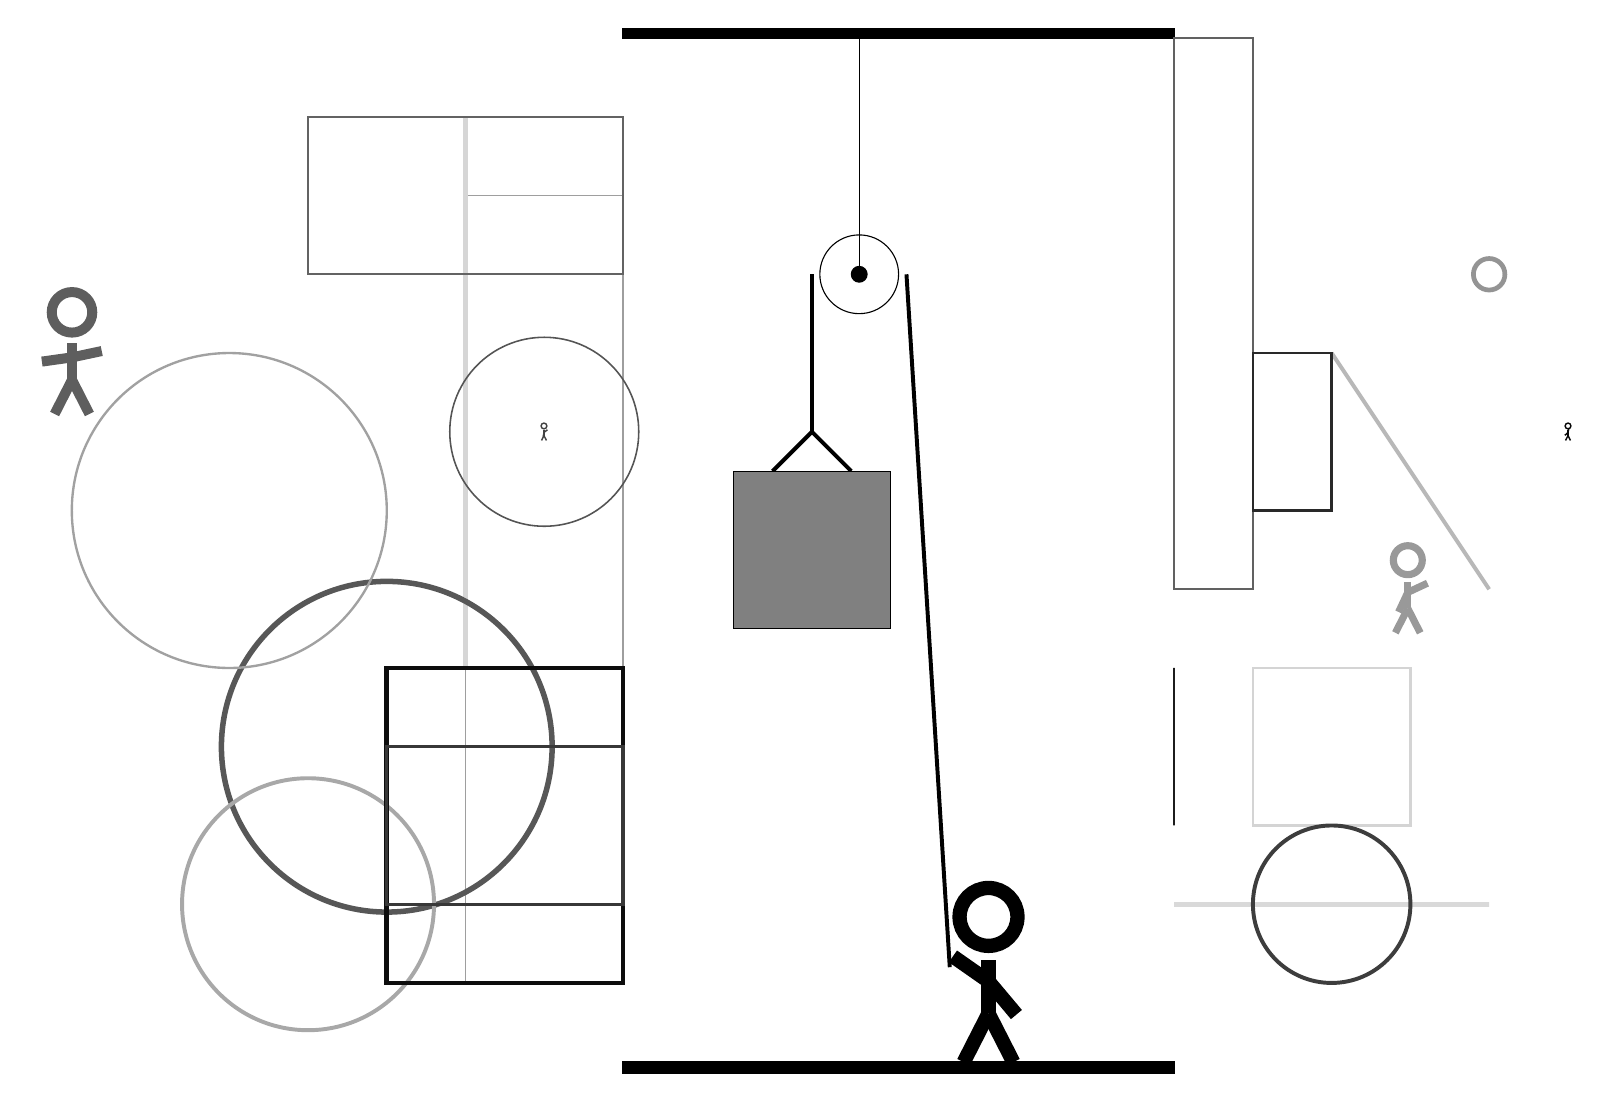
\begin{tikzpicture}
		%%%%% START %%%%%
		
		\draw[fill=black] (-2, 10) rectangle (5, 10.125);
		
		\draw (1, 7) circle (0.5);
		\draw[fill=black] (1, 7) circle (0.1);
		\draw (1, 10) -- (1, 7);
		
		\node[line width=0.6mm, color=black!40] at (8, 3) {\Strichmaxerl[5][65][25]};
		
		\draw[line width=0.3mm, color=black!62] (5, 3) rectangle (6, 10);
		\draw[line width=0.2mm, color=black!38] (-4, -2) rectangle (-2, 8);
		\draw[line width=0.5mm, color=black!28](7, 6) -- (9, 3);
		\draw[line width=0.6mm, color=black!16] (-4, 2) rectangle (-4, 9);
		\draw[line width=0.6mm, color=black!15] (5, -1) rectangle (9, -1);
		
		\node[line width=0.7mm, color=black!74] at (-3, 5) {\Strichmaxerl[1][80][37]};
		\draw[line width=0.3mm, color=black!17] (6, 0) rectangle (8, 2);
		\draw [line width=0.5mm, color=black!76](7, -1) circle (1.0);
		
		\draw [line width=0.7mm, color=black!66](-5, 1) circle (2.1);
		
		\draw [line width=0.6mm, color=black!42](9, 7) circle (0.2);
		\draw [line width=0.5mm, color=black!34](-6, -1) circle (1.6);
		\draw [line width=0.2mm, color=black!67](-3, 5) circle (1.2);
		
		\draw[line width=0.6mm, color=black!95] (-2, 2) rectangle (-5, -2);
		\draw[line width=0.4mm, color=black!78] (-2, 1) rectangle (-5, -1);
		\draw[line width=0.3mm, color=black!84] (6, 4) rectangle (7, 6);
		\draw[line width=0.3mm, color=black!61] (-2, 7) rectangle (-6, 9);
		\draw [line width=0.3mm, color=black!37](-7, 4) circle (2.0);
		\node[line width=0.2mm, color=black!63] at (-9, 6) {\Strichmaxerl[7][8][12]};
		
		\node[line width=0.5mm, color=black!97] at (10, 5) {\Strichmaxerl[1][43][78]};
		\draw[line width=0.3mm, color=black!89] (5, 0) rectangle (5, 2);
		
		\draw[line width=0.5mm] (-0.1, 4.5) -- (0.4, 5.0) -- (0.9, 4.5);
		\draw[fill=black!50] (-0.6, 4.5) rectangle (1.4, 2.5);
		
		\draw[line width=0.5mm] (0.4, 7) -- (0.4, 5.0);
		\centerarc[line width=0.5mm](1, 7)(0:180:0.6);
		\draw[line width=0.5mm](1.6, 7) -- (2.15, -1.8);
		
		\node at (2.6, -1.9) {\Strichmaxerl[10][-35][-50]};
		
		\draw[fill=black] (-2, -3) rectangle (5, -3.15);
		
		%%%%% END %%%%%
	\end{tikzpicture}
\end{document}